\newpage
\hypertarget{subSec:setupParser}{}
\subsection{Setting up the Parser}
\genHeader

The final thing our transformation needs in order to translate from a textual instance into a model is an ANTLR parser/unparser tool.

\begin{itemize}

\item[$\blacktriangleright$] Right-click on \texttt{DictionaryCodeAdapter} and navigate to ``eMolfon/ Add Parser/Unparser''
(Fig~\ref{eclipse:contextParser}).

\vspace{0.5cm}

\begin{figure}[htpb]
\begin{center}
  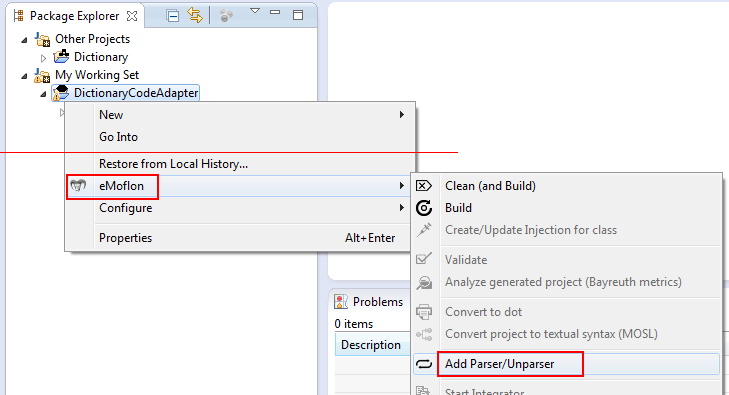
\includegraphics[width=0.8\textwidth]{eclipse_contextAddParserUnparser}
  \caption{figureCaption}
  \label{eclipse:contextParser}
\end{center}
\end{figure}


\item[$\blacktriangleright$] In the parser settings window, enter \texttt{dictionary} as the \texttt{File extension}, and confirm the \texttt{Create Parser},
\texttt{Create Unparser}, and \texttt{ANTLR} options are selected as the corresponding technology for each case (Fig~\ref{eclipse:wizardParser}). Affirm by
pressing \texttt{Finish}.

\begin{figure}[htpb]
\begin{center}
  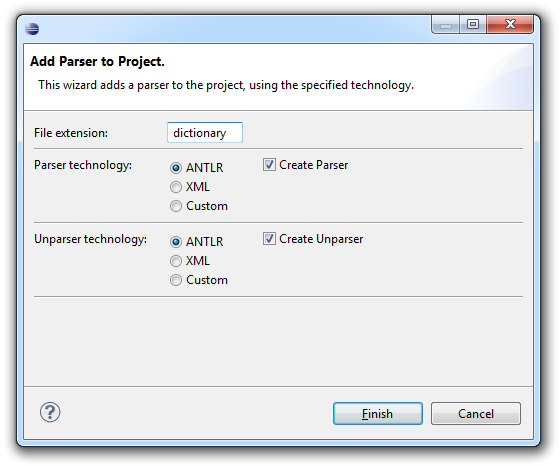
\includegraphics[width=0.8\textwidth]{eclipse_wizardParser}
  \caption{figureCaption}
  \label{eclipse:wizardParser}
\end{center}
\end{figure}

\vspace{0.5cm}

\item[$\blacktriangleright$] If everything was installed and completed without error, parser and unparser stubs should generate and appear in the \texttt{src}
package, where \texttt{ANTLR} automatically built the corresponding Java packages as depicted in Fig.~\ref{eclipse:generatedParser}. In addition, a new
\texttt{in} folder should appear under \texttt{instances} which will store any source text files.

\begin{figure}[htpb]
\begin{center}
  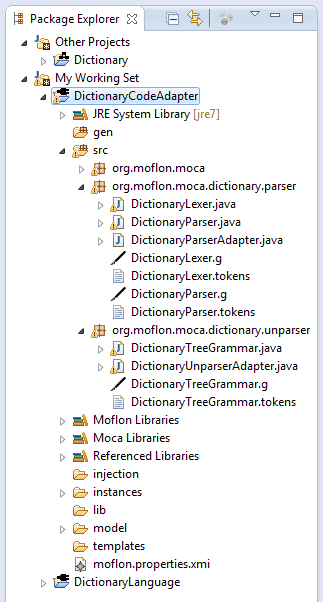
\includegraphics[width=0.4\textwidth]{eclipse_generatedParser}
  \caption{figureCaption}
  \label{eclipse:generatedParser}
\end{center}
\end{figure}

\vspace{0.5cm}

\item[$\blacktriangleright$] Your workspace is now ready to go!

\end{itemize}
